\documentclass[a4paper]{book}
\usepackage{extarrows}
\usepackage{amsmath,amsthm}
\usepackage{amsmath}
\usepackage{amssymb}
\usepackage{amsfonts}
\usepackage{answers}
\usepackage{eufrak}
\usepackage{eucal}
\usepackage{fancyhdr}
\usepackage{graphicx}
{\setlength\arraycolsep{2pt}
\usepackage{mathrsfs}
\usepackage{graphicx,fancyhdr}
\usepackage{graphicx} 
\graphicspath{ {./images/} }
\usepackage{CJKnumb}
\usepackage{titlesec}
\titleformat{\chapter}{}{}{0em}{\bf\huge}
\usepackage{amsthm}
\usepackage{cite}
\usepackage[utf8]{inputenc}
\usepackage[colorlinks,urlcolor=blue,citecolor=blue,linkcolor=blue]{hyperref}
\usepackage{tikz}
\usepackage{setspace}
\usepackage{xspace}
\usepackage{cite}

\newtheorem{theorem}{Theorem}%[section]
\newtheorem{lemma}[theorem]{Lemma}%[section]
\newtheorem{example}{Example}%[section]
\newtheorem*{remark*}{Remark}%[section]
\newtheorem*{note*}{Note}%[section]
\newtheorem{proposition}{Proposition}%[section]
\newtheorem{definition}{Definition}%[section]
\newtheorem{conjecture}{Conjecture}%[section]
\newtheorem{corollary}{Corollary}%[section]
\newtheorem{problem}{Problem}%[section]
\newtheorem{condition}{Condition}%[section]

\renewcommand{\proofname}{\textbf{Proof}}

\newenvironment{ddd}{\begin{rmdef}\rm}{\end{rmdef}}                             
\newenvironment{eee}{\begin{rmexa}\rm}{\end{rmexa}}                             
\newenvironment{rrr}{\begin{rmrem}\rm}{\end{rmrem}}                                   
					                                        
\newenvironment{pf}[1][Proof]{\par\noindent{\em #1}. }{\hfill\framebox(6,6)\par\medskip}

\usepackage{geometry}
 \usepackage[normalem]{ulem}
%\renewcommand{\baselinestretch}{1.5}

\geometry{left=3.5cm,right=3.5cm,top=2.5cm,bottom=2.5cm}

\newcommand{\Poincare}{Poincar\'e\xspace}
\newcommand{\Holder}{Hölder}

\usepackage{graphicx} %picture
\usepackage{float} %picture
\usepackage{subfigure} %picture

\usepackage[nottoc,notlot,notlof]{tocbibind}
%Hölder
%\renewcommand{\baselinestretch}{1.5}
\let\cleardoublepage\clearpage
\begin{document}

\begin{titlepage}\phantom{|}\vspace{0.75in}
\begin{center}
    \underline{THE ISOPERIMETRIC PROBLEM}
\end{center}
\begin{center}
    \underline{}
\end{center}
\vspace{1.5in}%{2.0in}
\begin{center}
    Dissertation submitted at the University of Leicester \\
    in partial fulfilment of the requirements for \\ 
    the degree of Bachelor of Science of Mathematics\\
\end{center}
\vspace{.5in}
\begin{center}
    by
\end{center}
\vspace{.5in}
\begin{center}
    Steven Cheung \\
    Department of Mathematics \\
    University of Leicester \\
\end{center}
\vspace{0.5in}
\begin{center}
    May 2024
\end{center}
\end{titlepage}

\tableofcontents
\thispagestyle{empty}
\chapter*{Declaration}                % The * means no number for this chapter
\pagenumbering{arabic}
\addcontentsline{toc}{chapter}{\hspace{0.2in}Declaration}
All sentences or passages quoted in this project dissertation from other
people's work have been specifically acknowledged by clear cross referencing
to author, work and page(s).  I understand that failure to do this amounts
to plagiarism and will be considered grounds for failure in this module and
the degree examination as a whole.


\bigskip

\noindent
Name: Steven Cheung


\bigskip

\noindent
Signed:


\bigskip

\noindent
Date:


\chapter*{Abstract}
\addcontentsline{toc}{chapter}{\hspace{0.2in}Abstract}
In general, we want the maximum area whose boundary has a specific length. 
\newline
\newline
For the 2-dimensional case.
\newline
\newline
For the 3-dimensional.
\newline
\newline
For the $n$-dimensional.
\newline
\newline
Manifolds?


\chapter*{Introduction}
\addcontentsline{toc}{chapter}{\hspace{0.2in}Introduction}
short intro to the problem
\section*{Historical Notes}
\addcontentsline{toc}{section}{\hspace{0.2in}Historical Notes}
Isoperimeter, isos which is ancient Greek for equal and perimetron for perimeter. The isoperimetric perimetric problem, even though not properly formalized, was already thought about. I'm talking about the legend of Dido. To begin, I'd like to quote Virgil
\begin{center}
    \begin{quote}
        At last they landed, where from far your eyes
        May view the turrets of new Carthage rise;
        There bought a space of ground, which Byrsa call'd,
        From the bull's hide they first inclos'd and wall'd.
    \end{quote}
    (Aeneid, Dryden’s translation)
\end{center}
Virgil's version has it that Dido, daughter of the king of Tyre, fled home after her brother killed her husband. Dido ended up on the north coast of Africa, where she bargained to buy as much land as she could enclose with an oxhide. Thus, she cut the hide into thin strips, presumably met and solved enclosing the largest area with a given perimeter - the isoperimetric problem. Dido may have been clever enough and chose an area by the coast to exploit the shore as part of the perimeter. But this mostly spoils the purity of posed problem. Kline concludes ~\cite{kline1985mathematics}. The Aeneid was written between 29 and 19 B.C. so it is clear that the isoperimetric problem has been known since at least that time period.
\begin{figure}[h]
    \begin{center}   
        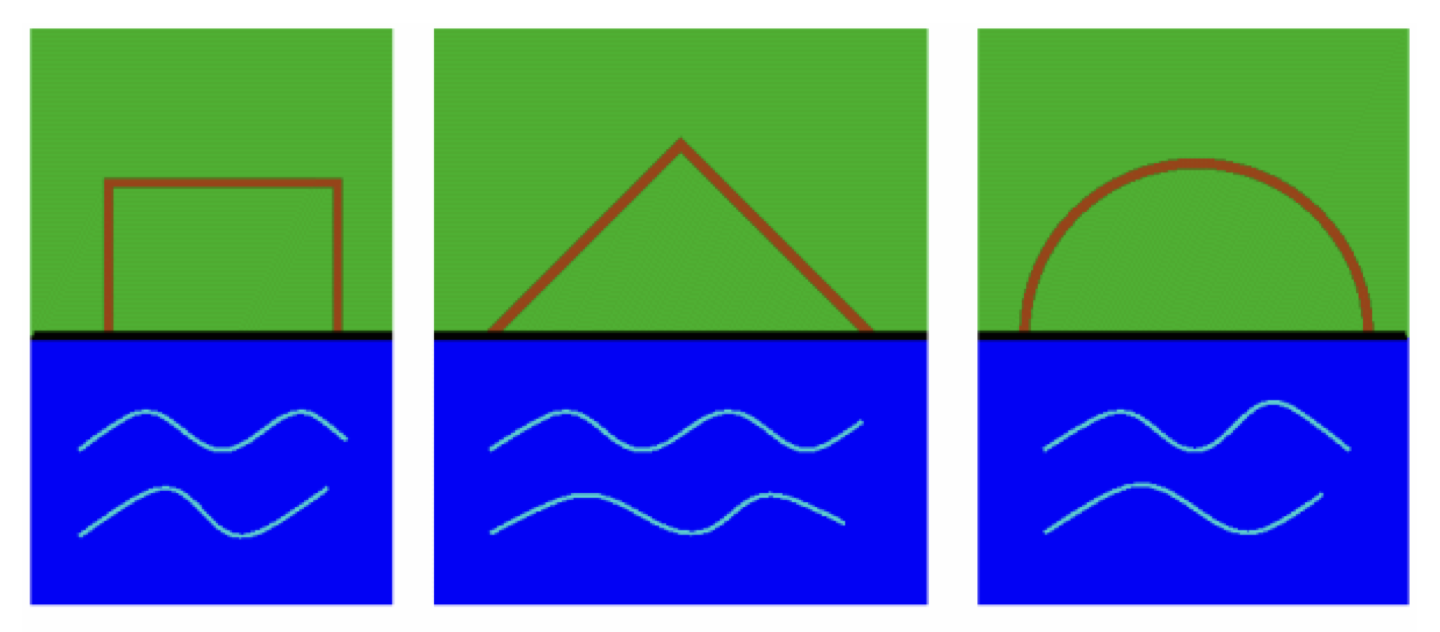
\includegraphics[width=100mm]{dido_1}
        \caption{Representations of areas bounded by common shapes of the same perimeter. The semicircle, answer to Dido's problem which contains the greatest area. Image from~\cite{demjanenko2008isoperimetric}.}
    \end{center}
\end{figure}

Since ancient Greece, around 100B.C., people has long considered that of all the planes closed curve with equal perimeters, which bounds the greatest area? As they wanted to measure the size of islands by timing how long it takes to circumnavigate the entire island. Proclus, a classical mathematician, mocked geometers for "measuring the size of a city from the lengths of its walls". To the common person of antiquity, two shapes with equal perimeter may have different areas. Interestingly, some individuals exploited this misconception to defraud others of land. Considerably more amusing, these con artists were viewed as liberal which demonstrates how unnatural the idea of shapes with a similar edge having different regions was to the old Greeks.

The Greek have pretty much solved it, by their standards. Zendorus was an ancient Greek mathematician from around $200B.C.$ to $120B.C.$. Zendorus had proved that a circle has greater area than any polygon with the same perimeter. Most of his work was lost. Fortunately, parts of his work survived through references by Pappus and Theon of Alexandria.

\section*{Important Preliminaries}
\addcontentsline{toc}{chapter}{\hspace{0.2in}Important Preliminaries}
(to do: find a good book to give the proof of the Jordan Curve theorem ,or from papers)
We will take for granted the Jordan Curve Theorem
\begin{theorem}[Jordan Curve Theorem]
    A simple closed curve in the plane divides the plane into two regions, one compact and one non-compact, and in the common boundary of both regions
\end{theorem}
\begin{note*}
    When we talk of the region bounded by a simple closed curve in the plane, we always mean the compact region
\end{note*}
---
(to do: change the 3 def below to more rigorous ones, ideally from books)
\begin{definition}
    A closed curve, is a curve that changes direction but does not cross itself whilst changing direction.
\end{definition}
\begin{definition}
    A simple curve, is a curve that changes direction but does not cross itself whilst changing direction.
\end{definition}
The two definitions, above, are vital into understanding the main theorem.
\begin{definition}
    A function is bounded if $\exists M \in \mathbb{R}$ such that $\left| f(x) \right| \leq M$.
\end{definition}
\begin{definition}
    Let $X$ be a topological space and $A \subset X$. An open cover for $A$ is a family $\{U_\lambda\}_{\lambda\in I}$ of open subsets of $X$ such that
    \begin{center}
        $A \subset \cup_{\lambda\in I}{U_\lambda}$
    \end{center}
    An open cover is called finite if $\|I\|<\infty$. If $\{U_\lambda\}_{\lambda\in I}$ is an open cover for $A$ and $J \subset I$ is such that $A\subset\cup_{\lambda\in J}{U_\lambda}$, then $\{U_\lambda\}_{\lambda\in J}$ is called a subcover of $\{U_\lambda\}_{\lambda\in I}$.
\end{definition}
\begin{definition}
    A subset $A \subset X$ of a topological space called compact if every open cover of $A$ has a finite subcover. A space is called compact space if it is a compact subset of itself.
\end{definition}
\begin{definition} (Heine-Borel Theorem)
    A set in $\mathbb{R}^n$ is said to be compact if it is closed and bounded.
\end{definition}


\chapter{The Isoperimetric Theorems for 2D, 3D and $n$D Cases}
\section{2 Dimensional Case (Plane)}
\begin{theorem}
    Let $C$ be a simple closed curve in the plane with length $L$ and bounding a region of area $A$ . 
    Then $L^2 \leq 4\pi A$ with equality if and only if $C$ is a circle.
\end{theorem}
The circle therefore bounds the biggest area among all simple closed curves in the plane with a given length.
\subsection{Unpacking Steiner's proof}
The proof that I will be unpacking and taking a closer look at will be from the book (reference the book here), and is credited by them to Jakob Sternier. Packed and concise proof from ~\cite{gluck2012isoperimetric}
\begin{proof}
    We will begin the proof by assuming the solution exists
\end{proof}

\section{3 Dimensional Case (Sphere)}

\section{$n$ Dimensional Case ($\mathbb{R}^n$)}

\chapter{Manifolds}

\bibliography{The-Isoperimetric-Problem-References}
\bibliographystyle{unsrt}
\end{document}